\section{Solution Description}

\subsection{Design Principles}

SPLA library is designed in the way to maximize potential library performance, to simplify its implementation and extensions, and to provided to the end-user verbose, but effective interface allowing customization and precise control over operations execution. This ideas are captured in the following principles.

\begin{itemize}
    \item \textit{DAG-based expressions}. User constructs a computational expression from basic nodes and uses oriented edges to describe data dependencies between these nodes. 
    \item \textit{Automated hybrid-storage format}. Library uses internally specialized preprocessing to format data and automate its sharing between computational nodes.
    \item \textit{Automated multi-GPU scheduling}. Computational work is automatically scheduled between available devices for execution. Scheduling order, dependencies and granularity are defined from DAG expression, submitted by user.
    \item \textit{Customization of primitive types and operations}. Underlying primitives types and functions, which operates on them, can be customized by user. Customization process does not requires library re-compilation. 
    \item \textit{Exportable interface}. Library has C++ interface with an automated reference-counting and with no-templates usage. It can be wrapped by C99 compatible API and exported to other languages, for example, in a form of a Python-package.
\end{itemize}

\subsection{Architecture Overview}

Library general execution architecture is depicted in Fig.~\ref{fig:architecture}. As an input library accepts expression composed in the form of a DAG.
Nodes represent fundamental operations, such as matrix-matrix multiplication. 
Links describe dependencies between nodes.
Expression execution is \textit{asynchronous}. 
User can block and wait until its completion, or without blocking probe the expression until it is either \textit{completed} or \textit{aborted}. 

Expression is transformed into a task graph. 
Task graph is submitted for execution to the task manager. 
Each task is processed by specialised \textit{NodeProcessor}, capable of processing particular node type.
Each task, when executed, is split dynamically into a set of parallel sub-tasks. 
Each sub-task is processed by specialized \textit{Algorithm}, which is capable of processing input blocks of matrices or vectors in particular storage formats with concrete set of options. \textit{NodePorcessor} and \textit{Algorithm} are selected at runtime from a registry of available set based on properties and arguments of the expression. 
Thus, it allows precise processing and optimization of edge-cases.

Granularity level of sub-tasks is defined by the structure of underlying processed primitives. 
Target device for execution is automatically assigned for the sub-task based on expression and node parameters. 
Currently, the uniform distribution for assignment is used, 
what should work good on large scale of computationally similar sub-tasks.

\begin{figure}[t]
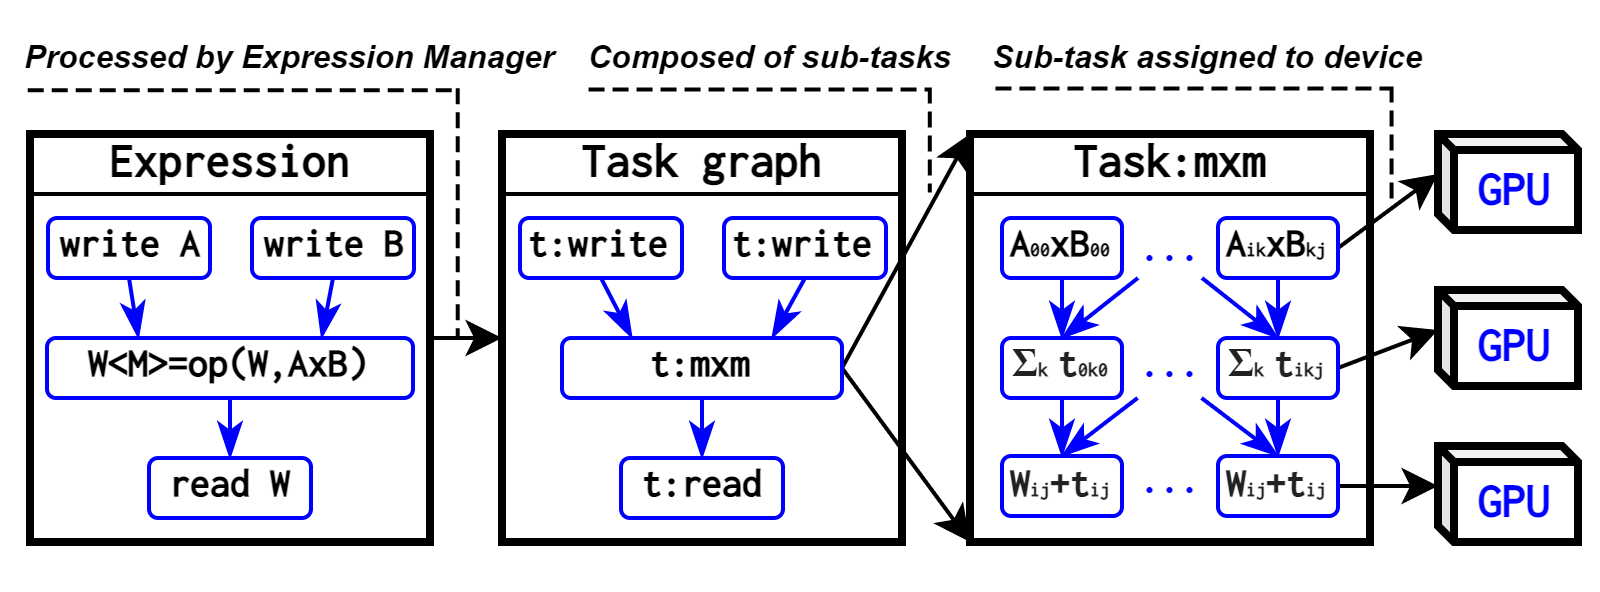
\includegraphics[width=0.99\linewidth]{figures/library_architecture.png}
\caption{Library expression processing architecture.}
\label{fig:architecture}
\end{figure}
    
\subsection{Matrices and Vectors}

Library provides general \textit{M-by-N Matrix} and \textit{N Vector} primitives.
Underlying primitives types is specified by \textit{Type} object. 
Internally primitives are stored in a hybrid storage in a form of two- or one- dimensional blocks' grid respectively. 
Each block is empty (not stored) or store some data in any format. Blocks are immutable, they can be safely shared across computational devices.

Currently only COO blocks are supported. Format choice is motivated by its simplicity and easy of implementation. 
Other formats, such as CSR, CSC, DCSR, Dense, etc. can be added to the library by either implementation of formats convertation or by the specialization of \textit{Algorithm} for concrete format.

\subsection{Algebraic Operations}

Library supports all commonly used linear algebra operations, such as \textit{mxm}, \textit{vxm}, \textit{eadd}, \textit{reduce}, \textit{transpose}. 
More operations coming later, since library still in development.
Interface of operations is designed in similar fashion as GraphBLAS ones. 
It supports \textit{masking}, \textit{accum} of the result, \textit{add} and/or \textit{mult} user-functions specification, and \textit{descriptor} object for additional operation tweaking.

\subsection{Implementation Details}

Library uses OpenCL 1.2 API as underlying compute API. 
Boost Compute~\cite{10.1145/2909437.2909454:boost:compute} is utilized as a high-level library on top of the OpenCL functionality. 
It provides thread-safe kernel caching, meta-kernel programming, and a set of basic parallel primitives such as \textit{device vector}, \textit{sort}, \textit{reduce}, \textit{scan}, etc. which was extended further to meet this project requirements.
Taskflow~\cite{Huang2022TaskflowAL} is used as tasking library. It supports task-dependencies and dynamic tasking, utilized in order to create and execute sub-tasks. 

User-defined \textit{Types} are represented as POD-structures, and handled by the library as a fixed-size sequences of bytes.
User-defined \textit{Functions} are effectively textual strings with OpenCL code, injected into generalized meta-kernels.
Library has a number of predefined types, such as \textit{signed/unsigned integers}, \textit{floating point} types, and a set of common operations, such as \textit{arithmetic}, \textit{logic}, \textit{first/second}, etc.

For particular blocked \textit{vxm} and \textit{mxm} \textit{Algorithms} implementations ESC algorithm~\cite{10.1145/2699470:esc:algo} for COO blocks is employed. 
Element-wise addition and masking are based on tiled GPU Merge Path~\cite{inproceedings:gpu_merge_path} algorithm. 
The code is generalized and is written in a form of meta-kernels, so actual functions for elements reduction or multiplication are injected later.
Kernel compilation is done on demand if no previously cached entry present.

